% !TEX root = /home/simon/repos/p5report/main.tex
% The preamble contains command definitions, macros and the like; 
% All the things that must be defined before \begin{document}.
\documentclass{proj-report}


% Adds support for full page background picture
\usepackage[contents={},color=gray]{background}

%%% Tables %%%
\usepackage{tabularx}
\usepackage{xltabular}

%%% Adjust page %%%
\usepackage{changepage} % Allows for adjustment of requirements table page.
\usepackage{lscape}     % Pages can be turned (landscape).
\usepackage{pdflscape}

%%% Bibliography %%%
%Currently uses BibTeX.
\bibliographystyle{plain}

%%% Hyperref %%%
\hypersetup{%
	pdfpagelabels=true,%
	plainpages=false,%
	pdfauthor={Author(s)},%
	pdftitle={Title},%
	pdfsubject={Subject},%
	bookmarksnumbered=true,%
	colorlinks=false,%
	citecolor=black,%
	filecolor=black,%
	linkcolor=black,% you should probably change this to black before printing
	urlcolor=black,%
	pdfstartview=FitH%
}



% Input the title and such for the title page
\title{Extension of Ecdar:Reveaal}
\subtitle{Eliminating clock redundancy}
\projectgroup{cs-22-sw-05-15}
\author{Simon \and Bimon \and Limon}
\date{Fall 2022}
\participants{\parbox[t]{0.5\textwidth}{%
Alexander Skytt Steffensen\\
Jens Emil Fink Højriis\\
Kira Stæhr Pedersen\\
Magnus Jørgensen Harder Christensen\\
Simon DeLauren Laursen\\
Thomas Krogh Lohse
}}
\supervisor{Martijn Angelo Goorden}
\department{Department of Computer Science}
\abstract{abstract}
\theme{Multiproject -- Ecdar}

\begin{document}
% Inserts the front page. You could change this to a custom front page.
\frontpage
\indexpage

\tableofcontents

\include{00-preface/00-preface-main-tex}
\chapter{Introduction}
This project report details the implementation of clock reduction in ECDAR. The first section will introduce ECDAR as a model checking engine and explain the major concepts that are relevant to the project. The second section will present scrum as the framework used for collaboration. The third section will introduce the ECDAR-SW5 organization and explain how six project groups were able to collaborate on the same project. Finally, the third section contains a glossary with all of the terminology that we use throughout the report.

\section{Model Checking}\label{sec:model-checking}

Systems nowadays are big and complex and consists of multiple components designed by independent teams \cite{ecdartheory}. Model checking is a method used in the software industry for years as a form of computer aided verification where logic is used for bug finding \cite{modelchecking_handbook}. A model checker takes a description of a system, known as a model, and a system specification. The model checker compares the model to the specification to check if it is satisfied by the model. If the model violates rules of the specification, the model checker produces a counter example that proves the model is indeed in violation of the specification  \cite{modelchecking_handbook}.



\def \commondisclaimer{\textit{The following section and its subsections are written in collaboration with other ECDAR project groups.}\vspace{1em}}
\section{Introduction to ECDAR}\label{sec:introduction-to-ecdar}
\textit{The following section and its subsections are written in collaboration with other ECDAR project groups.}\vspace{1em}

This section serves as an overview over the different concepts of ECDAR to provide a basic understanding of what ECDAR is, the purpose of ECDAR, its architecture, the technologies behind it, and what state ECDAR is currently in.

ECDAR stands for \textbf{E}nvironment for \textbf{C}ompositional \textbf{D}esign and \textbf{A}nalysis of \textbf{R}eal Time Systems.
ECDAR is a graphical tool to model real-time systems using timed input/output automata, and analyse these systems. 
This process is called model checking. 

%what
Model checking is a method of verifying that system models in the form of finite-state automata are correct \cite{modelchecking-handbook}. 
The bigger a model becomes, the harder it becomes to verify each edge case. 
Having computer-aided checking ensures that all edge cases are checked, where one can be forgotten if done by hand.

%why
What ECDAR is useful for is best described by an example \label{ECDAR:satellite}:

Imagine you are working for a space program and want to send a satellite into space.
You spent several months testing the system to make sure the model is correct and everything is working as intended.
The day after launch, you find a major issue in the system.
The satellite is already in space, and you cannot simply just update it, like you usually would with other systems. 
This is why ECDAR is a useful tool to model check systems, to make sure that a system's components works together as expected.

Model checking is a way of checking if a model is true to a given specification.
This is usually associated with hardware or systems that have a liveness, since validity of the life cycle needs checking.
There is also a need for certain safety requirements to ensure that there are no crashes or other obstacles throughout the life cycle.

It is important to model check a system to ensure that it behaves as intended.
In the above example with the faulty satellite, there are several, interdependent components.
If one of these components fail or are blocked, then it makes the entire satellite faulty.
% Take for instance the satellite example, it is a very complex hardware/system with a lot of functionality.
% The satellite itself has several components, which are dependent on each other.

By providing a tool that can both be reliable and productive at testing if a new system is true to a given specification, we can not only ensure correctness but also efficiency.

It does need to be noted that there still are some issues with using ECDAR as a tool for model checking.
ECDAR can try to guide the user as much as possible to make sure the specification is valid, but in the end, the user can still make a wrong specification.
%Also how efficient ECDAR is as a tool is dependent on what kind of algorithms are used, and the efficiency of the run-time.

%%ECDAR therefore tests the correctness of the model using timed I/O automata.
%% It parallelizes test-case generation and test execution to provide this significant speed-up.

To sum up, what the purpose of ECDAR is:
\begin{quote}
"[to integrate] conformance testing into a new IDE that now features
modelling, verification, and testing. The new tool uses model-based mutation testing, requiring only
the model and the system under test, to locate faults and to prove the absence of certain types of faults." \cite{Gundersen_2018}
\end{quote}




\subsection{Architecture}\label{sub:architecture}
ECDAR consists of four major systems as seen in \autoref{fig:ECDAR-architecture}.
There are the two engines, Reveaal and j-Ecdar, as well as the ECDAR GUI, and a test framework as seen in \autoref{fig:ECDAR-architecture}. 
The GUI and the engines communicate through Protocol Buffers (Protobuf) and gRPC (\textbf{G}oogle \textbf{R}emote \textbf{P}rocedure \textbf{C}all) as indicated by the arrows.
\begin{figure}[H]
    \centering
    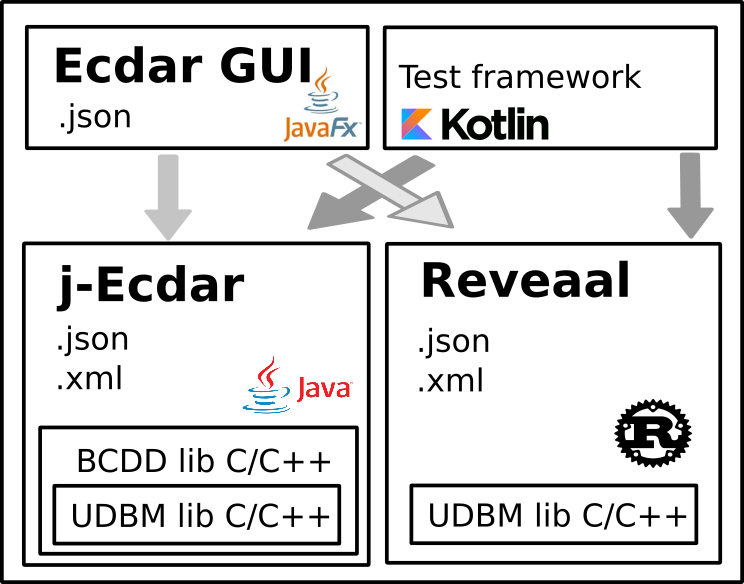
\includegraphics[width=0.75\textwidth]{common/figures/ArchOverview.png}
    \caption{The architecture of ECDAR visualized \cite{ECDARNET}.}
    \label{fig:ECDAR-architecture}
\end{figure}
% Figure old, get new

The graphical user interface (\textbf{GUI}) is written in JavaFX \cite{ECDARNET}  which is a graphics and media library for Java. 
The interface provides the tools which enables the user to model their real time systems. The GUI sends queries to the engines through gRPC using Protobuf. 
%This is illustrated by the arrows going from the Ecdar GUI component to the j-Ecdar and Reveaal components, as seen in \autoref{fig:ECDAR-architecture}. 
The gRPC and Protobuf frameworks have the advantage of being cross platform and work across languages \cite{gRPC}\cite{google_protocol_nodate}, simplifying the integration process and making it easy to use.

ECDAR runs on two verification engines: j-Ecdar and Reveaal. 
The purpose of having two different engines is to make the whole platform more reliable. 
With two engines their results can be compared which will help ensure correctness in both engines.
The j-Ecdar component is an engine written in Java.
The main priorities for this engine are readability and correctness, and, as stated on ECDAR's homepage: "no effort is put into optimizing the code for speed" \cite{ECDARNET}.
In contrast to this, the Reveaal engine is intended to be fast and parallelizable. 
Recently, the libraries which the engine uses have been rewritten in Rust from C/C++, with the intention of implementing multithreading. 

ECDAR makes use of a testing framework written in Kotlin. 
The testing framework uses a collection of test cases to test both of the engines. 
The testing framework is vital to perform conformance testing between j-Ecdar and Reveaal as well as automated performance testing and hand-designed test cases. 
\subsection{The current state of ECDAR}\label{sub:the-current-state-of-ecdar} %This was written quite fastly ;)
To further illustrate what ECDAR is and how far it has been developed, we will go through the tool in this section, a screenshot of which can be found in \autoref{fig:ECDAR-gui}. 
The version of ECDAR described here is ECDAR version 2.3.3. %downloaded from \href{https://www.ecdar.net/download/}{ecdar.net/download/}.

The GUI is mainly split up into three parts, as seen in \autoref{fig:ECDAR-gui}: The different components in the project to the left, the currently selected automaton in the middle, and the queries to the right.
The GUI also has a top bar, which is self-explanatory, and will therefore not be described.
However, an interesting thing to mention is how to open a project using the \textit{File} tab.
An existing project is opened by selecting the folder containing three folders with the names: \textit{Components}, \textit{Systems} and \textit{Tests}.

\begin{figure}[H]
    \centering
    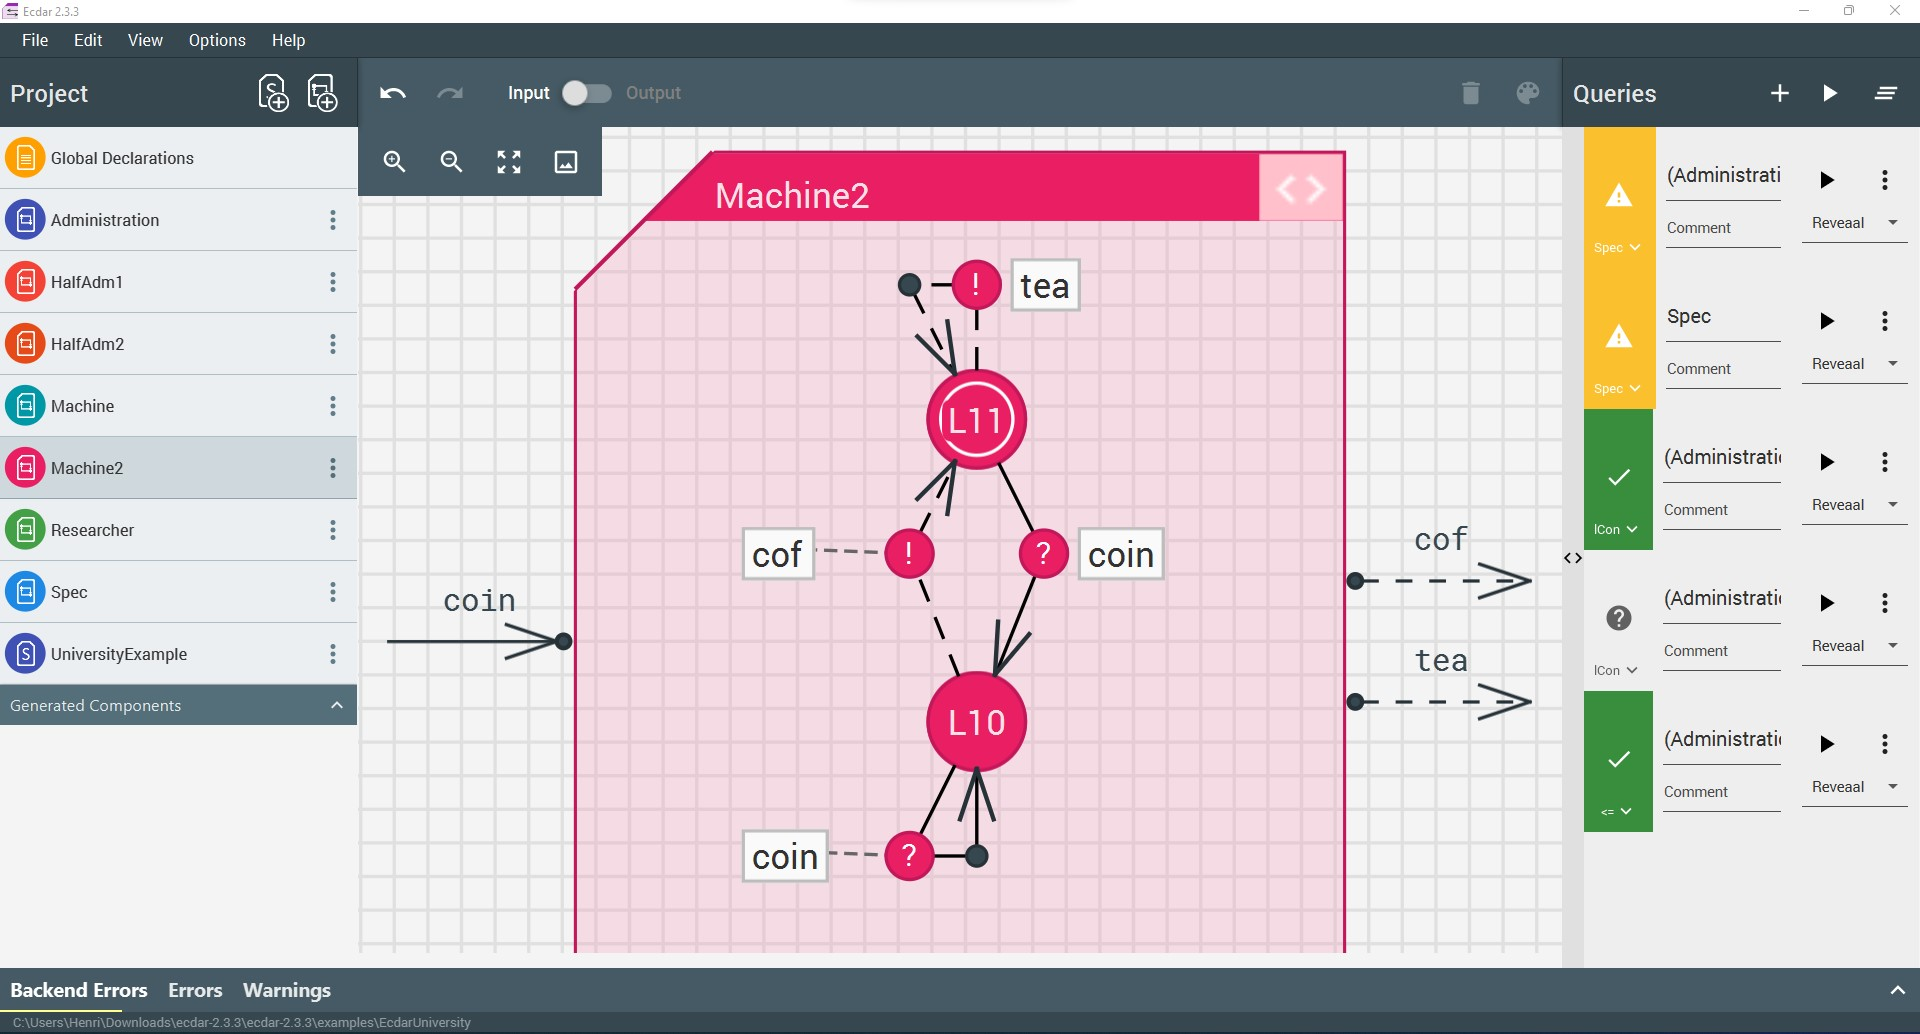
\includegraphics[width=1\textwidth]{common/figures/ecdar-overview.jpg}
    \caption{A screenshot of the ECDAR GUI.}
    \label{fig:ECDAR-gui}
\end{figure}

%\subsubsection{The component panel}
The panel on the left of \autoref{fig:ECDAR-gui} contains an overview of the components and specifications. 
Positioned at the top of this tab, to the right of "Project"-text box, are the two buttons for creating new models and new specifications under the currently opened project.
ECDAR allows the user to create a type of automaton called \textbf{T}imed \textbf{I}nput \textbf{O}utput \textbf{A}utomata. 
In the left panel, the component \textit{Machine2} is selected, which is displayed in the middle of the GUI.
This example is of an automaton that models a coffee machine.
It takes \texttt{coin} as input, since the arrow is solid, and the automaton outputs \texttt{cof} and \texttt{tea}, as shown by the dashed arrows on the left side of the automaton.
Inside the red box, the \texttt{L11} location is marked as the start state, which is indicated by the circle.
A solid arrow through a small circle with a question mark represent an output. 
Likewise, if the arrow is dashed and the small circle contains an exclamation mark, it represents an input.
This concludes the possibilities regarding input and output.

\autoref{fig:ECDAR-guard} contains an automaton which uses time as well as input and output.
This is done by using a clock, represented as the variable y.
\begin{figure}[H]
    \centering
    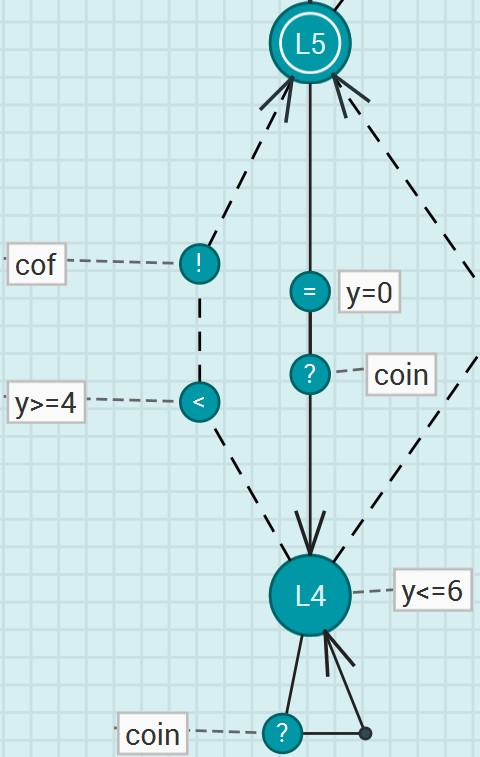
\includegraphics[width=0.3\textwidth]{common/figures/ecdar-guards.jpg}
    \caption{A screenshot of an automaton with a guard and an invariant.}
    \label{fig:ECDAR-guard}
\end{figure}

The transition with the small circle containing the assignment is an \textit{update} that resets the clock.
The small circle containing a "$>=$"-sign is a \textit{guard}, which can be thought of as a restriction that must be satisfied in order to take this action/transition.
Finally the \texttt{L4}-location contains an \textit{invariant} \texttt{y<=6}, which must be satisfied. 
In this case, it means the automaton cannot be in the location if the clock value exceeds the value of 6.

The rightmost panel displays the queries to be performed. 
Queries are sent to an engine, which can be selected in the drop-down menu, one of which can be seen in the bottom-right corner of \autoref{fig:ECDAR-queries-panel}. 
\begin{figure}[H]
    \centering
    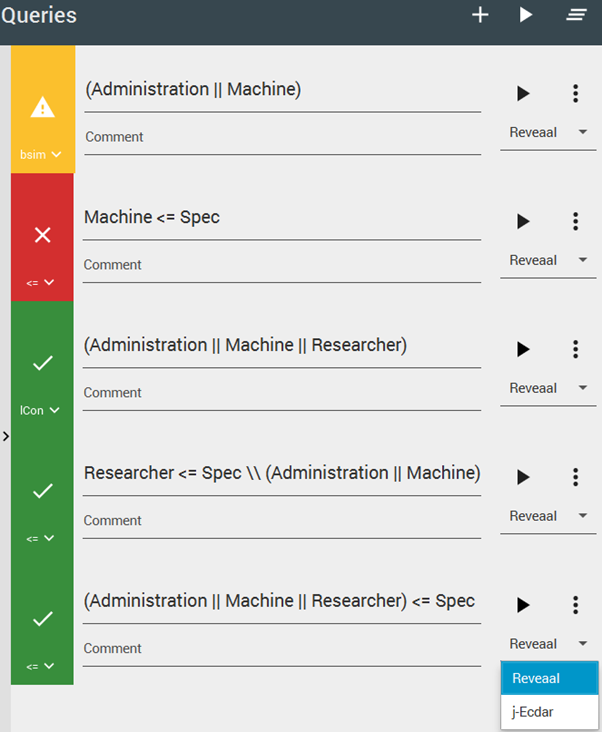
\includegraphics[width=0.6\textwidth]{common/figures/right-panel.png}
    \caption{A screenshot of the right panel of the GUI, which displays the queries.}
    \label{fig:ECDAR-queries-panel}
\end{figure}
To send the queries to be checked, the button with the ``play'' icon must be pressed.
Afterwards the result can be viewed on the left side of the panel in the form of an icon and a color. 
The result of the query in the top of \autoref{fig:ECDAR-queries-panel} is an error, which means the engine could not perform the query. 
An error message can be seen by placing the mouse over the icon, which can be used to troubleshoot why this error occurred.
The "Machine$<=$Spec" query was performed, but the result was false, which means the \texttt{Machine} model does not refine the specification named \texttt{Spec}, as illustrated by the red color and a cross.
The rest of the queries were performed without errors, and all proved true.
The text boxes use a special syntax to specify a combination of models, operators, and specifications to be checked.

\begin{figure}[H]
    \centering
    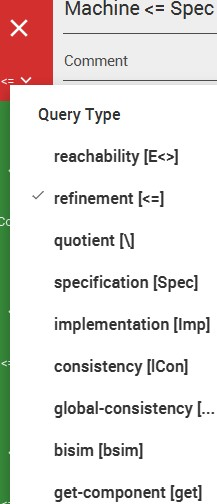
\includegraphics[width=0.25\textwidth]{common/figures/check-type.jpg}
    \caption{A screenshot of drop-down menu with the query types.}
    \label{fig:ECDAR-query-types}
\end{figure}

The type of the query to be performed is chosen in the drop-down menu underneath the icons. 
The drop-down menu with the types of queries that can be chosen, can be seen in \autoref{fig:ECDAR-query-types}.




\subsection{Timed Input/Output Automata}\label{sec:TIOA}
\emph{Timed Input/Output Automata}, abbreviated to TIOA, are basic automata with two extensions \cite{ecdartheory}. One of them being the notion of time. Time is tracked using clock variables, which can be used to make conditions on the system being in a location or performing an action. The second is having actions classified as either input or output actions. Input actions triggers from the outside, where output actions triggers from within. 

The formal definition of a TIOA is a tuple \cite{ecdartheory} $$(Loc, I_{0}, Act, Clk, E, Inv)$$  
where:

\begin{itemize}
    \item $Loc$ is a finite set of locations.
    \item $i_{0}$ is the initial location, so $i_{0} \in Loc$.
    \item $Act$ is a finite set of actions partitioned into inputs ($Act_{i}$) and outputs ($Act_{o}$).
    \item $Clk$ is a finite set of clocks.
    \item $E \subseteq Loc \times Act \times \mathcal{G} \times \mathcal{U} \times Loc$ is a set of edges.
    \item $Inv : Loc \mapsto \mathcal{B}(Clk)$ is a location invariant function. 
\end{itemize}

\subsection{Timed Input/Output Transistion Systems}\label{sec:TIOTS}

\emph{Timed Input/Output Transistion System}, TIOTS, is the semantic representation of TIOA and is used to analyze them, to ensure their correctness. TIOA are finite representations of TIOTS \cite{}. A TIOTS is a tuple \cite{}  $$(Q, q_{0}, Act, \rightarrow)$$

where:

\begin{itemize}
    \item $Q$ is a possibly infinite set of states.
    \item $q_{0}$ is the initial location, so $q_{0} \in Q$.
    \item $Act$ is a finite set of actions partitioned into inputs ($Act_{i}$) and outputs ($Act_{o}$).
    \item $\rightarrow \subseteq Q \times (Act \times \mathbb{R}_{\geq 0}) \times Q$ is a transition relation.
\end{itemize}

\subsubsection{Specification}
A TIOTS is a specification if all of it states are input enabled, this means that if $\forall i? \in Act_i : \exists q' \in Q$ which means that each state in a TIOA should be able to take input, at any time. i.e. $q \rightarrow^{i?} q'$\cite{}
\subsection{DBM}\label{sec:DBM}
In a TIOA it is crucial to keep track on the clocks and their guards and invariants. This can be done by the usage of \emph{Difference Bound Matrices} (abbreviated to DBM). This is the method Reveaal uses.
A DBM is used to represent \emph{zones};  convex spaces where a clock-invariant evaluates to true. The size of a DBM is $n+1 \times n+1$ where $n$ is the number of clocks in the model.
Each entry in a DBM is the a tuple $(a, \prec)$ where $\prec \in \hspace{-3pt} \{<, \leq\}$ and $a \in \mathbb{R} \cup \{ -\infty, \infty \}$ \cite{peron:hal-00189821, Joost:DBM19}. The tuple $(a, \prec)$ consists of $a$ which is a constant that sets the bound for the clock, where $\prec$ tells if the constant is inside the bound or not.
Given a DBM and entries row $i$ column $j$, the invariant can be interpreted as a logical conjunction of all entries $c_i - c_j \prec a$. 

In Equation \ref{eq:con} we see an example for a constraint, and the according DBM can be seen in Equation \ref{eq:DBM_ex} and the visualisation in Figure \ref{fig:DBM_ex}.
\begin{equation}\label{eq:con}
    x \geq 2 \wedge x \leq 6 \wedge y \geq 1 \wedge y \leq 5 \wedge x \leq y + 3 \wedge y \leq x + 1
\end{equation}
\begin{equation}\label{eq:DBM_ex}
    M = 
    \begin{bmatrix}
                 &&    x    &    y\\
          & (0, \leq) & (-2, <) & (-1, <)\\
        x & (6, <) & (0, \leq) & (3, <)\\
        y & (5, \leq) & (1, <) & (0, \leq) 
    \end{bmatrix}
\end{equation}

\begin{figure}[H]
    \centering
    \begin{tikzpicture}
        \coordSys{6}{5}
        \drawDBM{{(2,1), (2,3), (4,5), (6,5), (6,3), (4,1)}}{blue!25!white}
    \end{tikzpicture}
    \caption{A visuallisation of DBM $M$ with two clocks; $x$ and $y$}
    \label{fig:DBM_ex}
\end{figure}

One might notice that one DBM can only represent one guard/invariant, but in a large system with multiple edges and locations we need several. This is done by using \emph{Federations}, which is a collection of DBMs, capable of performing special operations on the DBMs such as finding the intersection between two DBMs, which corresponds to the zone of which both invariants evaluate to true. Federations can also be viewed as a union of zones \cite{ecdartheory, Rokicki_DBM}.
\subsection{Introduction to Clock Reduction}
When removing clocks from the TIOA, it is important to make sure that the clock is never checked or it is redundant. In Reveaal most of the time is spent on DBM operations. These operations are quadratic in the number of clocks, so removing clocks would decrease the size of the DBM and the number of operations.



\section{Agile Software Development} \label{sec:agile-software-development}
\commondisclaimer

This section gives an introduction to agile development in general, scrum will also be introduced as a specific agile framework. Planned development through the waterfall method will also briefly be introduced, as an alternative to the agile approach.
Before agile development, project management relied heavily on the waterfall method \cite{sommerville}. 
Waterfall entails planning everything before proceeding with development in stages.
Every stage is completed entirely before the next begins. 
This method can be useful when both the problem and implementation is clearly defined and unlikely to change during process. 
The problem with waterfall is that it has no mechanism for handling uncertainty \cite{sommerville}. 
Because we are working with a codebase, language as well as techniques that are completely new to most of us, we wish to stay open in our work strategy, so as to avoid getting stuck.
If the requirements change during development, the waterfall method cannot account for that.
%As it is possible for requirements to change during development, the waterfall model is not ideal for this particular project.
Agile development practices arose from a need for a development method that would solve the issues posed by waterfall.
Most importantly, it would lessen the cost of making changes to the specification late in the development process \cite{alancline}. 
The Agile Manifesto from 2001 outlines the values that agile development practices are supposed to support \cite{beck2001agile}. 
The first statement of the manifesto is: \say{Individuals and interactions over processes and tools} \cite{beck2001agile}.
Agile development is ideal for projects that require flexibility and communication, which makes it ideal for the Ecdar project. 
A potential disadvantage of agile development is lack of focus on documentation, which is something we must then be aware of throughout the project.
This statement concisely encompasses the change of focus from planning and strict application of well-defined procedures. 
Instead, the focus should be on delivering software that the user wants.

\subsection{Scrum} \label{sub:scrum}
Scrum is an agile framework that developers use to ensure a development process where \emph{Commitment, Focus, Openness, Respect, and Courage} is valued and practiced \cite{schwaber_sutherland_2022}. 
This subsection is heavy on the theory behind Scrum, so as to introduce the concept to the reader.
In subsequent chapters, the usage of Scrum for this particular project will be made clear.

%Scrum is a rugby term that describes a situation where \say{...the forwards from each team pack together, heads down and arms interlocked, and push against the opposing forwards in order to gain possession of the ball ...} \cite{oedscrum}.
%For development, this translates to a working framework where all \say{players} advances together as a team. 
%For this reason, an important aspect of Scrum is to assign roles to each \say{player}.

% Roles
\subsubsection{Roles}
The Scrum framework describes a team that consists of a \emph{Scrum Master}, a \emph{Product Owner}, and \emph{Developers}. 
These roles, described below, are all equally vital, and are not positioned in a hierarchy. 
Instead, everyone on the team is responsible for playing their part in the development and ensuring that working software is delivered. 
Scrum is based on having a small and nimble team that is still large enough to make significant progress during each sprint.
These teams should typically be less than 10 people \cite{schwaber_sutherland_2022}.

\paragraph{The Product Owner}
is responsible for maximizing the value created by the Scrum teams. 
It is also the Product Owner's responsibility to manage the \emph{Product Backlog} as well as developing and communicating what the \emph{Product Goal} is \cite{schwaber_sutherland_2022}. 

\paragraph{The Scrum Master}
is responsible for making sure the team is focused on reaching the goal and maintaining an environment where the Scrum values are upheld. This includes ensuring that the team follows the Scrum framework, removing obstacles for the team as well as facilitating the different Scrum events.
The Scrum master is not a manager, but a member of the team and is on equal terms with the rest of the team \cite{schwaber_sutherland_2022}.
 
\paragraph{The Developers}
make up the rest of the team members.
The developers are accountable for creating usable \emph{Increments} during the \emph{Sprint}. 
An Increment is a tangible step towards the \emph{Product Goal}, which meets the Definition of Done. 
Developers take part in creating the \emph{Sprint Backlog}, ensuring that \emph{Increments} adhere to the Definition of Done and adapting their daily plan in accordance with the current \emph{Sprint Goal} \cite{schwaber_sutherland_2022}.
The Definition of Done is described in \autoref{par:definition-of-done}.

\subsubsection{Scrum Artifacts}
The \emph{Product Backlog} is one of the three artifacts in Scrum, where the progress of the \emph{Product Backlog} is compared to the \emph{Product Goal}.
The product goal (also known as \say{commitment}) is a description of a future state for the product, typically its final form.
It is an ordered list that indicates which components of the product need to be improved as well as which definitions of features need to be made.
The list is used to delegate assignments between the Scrum groups for the upcoming \emph{Sprint}.
\emph{Refinement} of the \emph{Product Backlog} is a breakdown of the list, where the items are further defined into smaller and more precise items.
This is an ongoing event throughout the different \emph{Sprints}, slowly specifying and clarifying the \emph{Product Backlog} \cite{schwaber_sutherland_2022}. 

The second artifact is the \emph{Sprint Backlog}. 
This artifact is the set of \emph{Product Backlog} items the Scrum team has selected for the \emph{Sprint}. 
This list of items from the \emph{Product Backlog} is planned by and for the developers in the Scrum teams. 
Throughout the \emph{Sprint} the \emph{Sprint Backlog} is updated first during the during \emph{Sprint planning} and throughout the \emph{Sprint} and each time the Scrum team gains new knowledge about the problem or discover new issues \cite{schwaber_sutherland_2022}. 

The \emph{Increment} is the third and last artifact in Scrum, and it is a concrete stepping stone towards the \emph{Product Goal}.
An increment is created once a task from the product backlog meets the DoD. 
Every increment is thoroughly verified to ensure that all them work together, as each of them is an additive to the prior ones completed by the Scrum teams.
It is possible that multiple increments are created within a sprint.
An increment cannot be considered done if it does not uphold the criteria in the DoD\cite{schwaber_sutherland_2022}.

\paragraph{Definition of Done} \label{par:definition-of-done}
is a shared definition for when an \emph{Increment} meets the quality standards of the product and thereby describes when an \emph{Increment} is created.
This happens when an item from the backlog meets the definition.
The DoD, creates a shared transparency for the understanding of what have been completed as an \emph{Increment}.
When multiple Scrum teams works together, a mutual DoD must be defined \cite{schwaber_sutherland_2022}.
% Events
\subsubsection{Scrum Events}
The Scrum framework contains five events. 
These events are designed to enable transparency and create opportunities for course correction \cite{schwaber_sutherland_2022}.

\paragraph{The Sprint}
is a fixed length event, typically a month or less.
This event is where value is created. 
During the \emph{Sprint}, items from the \emph{Sprint Backlog} are turned into \emph{Increments} by the developers \cite{schwaber_sutherland_2022}.
The following events happen during a sprint and are done in the order they are described. 

\paragraph{Sprint Planning}
is the process where the Scrum team creates a plan for the sprint.
The plan should specify three things. 
Firstly, the plan should address why the sprint is valuable to the development of the product. 
Secondly, it should address which items from the product backlog will be added to the sprint backlog. 
The sprint backlog is the set of product backlog items the Scrum team has selected for the sprint. However depending on the product backlog, the selected items may need to undergo refinement before they can be turned into suitable tasks for the sprint backlog. 
Finally, the team should discuss how they will approach each backlog item and ensure that it will meet the DoD \cite{schwaber_sutherland_2022}.

\paragraph{Daily Scrum}
is a short meeting that is held each day, where the progress is inspected via a \say{three-question round} to clarify what each participant did the previous day, what they plan on doing this day, and whether there are any challenges to completing the day's work.
The goal of this event is to improve the group members' communication skills, helps identify challenges, and creates an opportunity for the team to share knowledge.
The daily scrum is also used to adapt or re-plan the work of the ongoing sprint \cite{schwaber_sutherland_2022}.

\paragraph{Sprint Review}
is the second to last event before a new sprint begins.
Its purpose is to inspect the outcome of the sprint to adjust the product backlog accordingly \cite{schwaber_sutherland_2022}.
Everyone involved with the project can participate in the sprint review (product owner, scrum master, developers, even customers, management and relevant developers from other projects).

\paragraph{Sprint Retrospective}
is the last event in the Sprint before a new sprint begins.
In a Sprint Retrospective, the team discusses how the processes and interactions during the Sprint helped or hindered the development process. 
Then, the team will discuss how it can improve its effectiveness and the quality of the outcome in the Sprint to come \cite{schwaber_sutherland_2022}.
The retrospective differs from the review in its focus; the retrospective (ideally) improves the work process moving forward, the review (ideally) improves the product.


\section{Collaboration}\label{sec:cooperation}
\commondisclaimer

\noindent This semester project specifically focuses on multi-project collaboration, which means that several project groups will be cooperating on the same project. 
Each project group functions as a Scrum team. 
In total, six project groups consisting of six members each will be collaborating to extend ECDAR further. 
Five of these groups will focus on further development of the Reveaal engine, while the last group will focus on developing the graphical user interface of ECDAR.

\subsection{The ECDAR-SW5 Organization}\label{sub:ecdar-organization}
To better orchestrate collaboration between all Scrum groups, it is essential to organize how communication will take place, as well as how we will distribute and evaluate work.
%There must be some kind of organization in order to orchestrate collaboration between all the project groups that are working on the ECDAR project. 
%Organisation is important because it establishes channels of communication, a distribution of the workload, and a process for evaluating the outcome of each stage in the development process.

Each of the project groups are themselves a Scrum team.
As Scrum is dependent on the teams being small, the organization must use an agile scaling framework.
Such a framework ensures distribution of the workload between the teams and that the output from each team can be integrated. 


As an organization, the ECDAR-SW5 organization found it crucial to consider its needs before picking a framework to implement.
Due to the requirements from Aalborg University as well as what is preferred within the six individual groups, each group must be self-managed and free to decide how they work internally.
From these requirements we decided that Scrum of Scrums was a good way of scaling our organization. Scrum of Scrums was chosen, as Scrum was already known, and preferred. The Scrum of Scrums framework allowed each team to still work as one team, while still providing teamwork across teams. Other possible solutions exist, we might have chosen to use eXtreme Programming, or any other agile framework. The choice of Scrum of Scrums, was made due to it being the most well known, and well understood method.
%This led us to choose to work in "Scrum of Scrums", allowing each group to work in their own way without sacrificing the teamwork that Scrum provides across the organization.

%As agile is very popular within some of the largest organizations in the world(SOURCE PLEASE), multiple different agile scaling frameworks have been invented. 

\subsection{Scrum of scrums}\label{sub:scrum-of-scrums}
Scrum of Scrums is a framework for scaling scrum across an organization. 
The ECDAR-SW5 organization uses Scrum of Scrums, as it allows each scrum team freedom to operate independently while providing a structure for communication \cite{spanner_scrum_nodate}. 

%In scrum of scrums we do not have daily scrums because the daily scrums is held in the smaller groups.
The daily scrum is a daily event, and because of that it would be impossible to get everyone together in the scrum of scrums every day for a daily scrum meeting.
Based on that we do not have daily scrums in the scrum of scrums.
%Working in scrum of scrums allows us as an organization to only hold daily scrum in each individual group, rather than across the entire organization.
%This simplifies the entire work process, ensuring focus. 
The key events in scrum of scrums are the sprint planning, sprint review, and sprint retrospective, and these events are handled by representatives of each group, which ensures that all groups have some insight into the overall process.
See \autoref{fig:scrum-of-scrums-events} for a more detailed look of the different events between scrum and scrum of scrums.

The multi-project is separated into two parts. 
There are five project groups working with the Reveaal engine, and one group working with GUI.
Each group has chosen a member to attend the scrum of scrums meetings as a representative of the group.
The reasoning for this was the number of members attending the meetings would get to big if every group member attended. 
The idea behind this was to keep the meetings as short as possible, and because of this, each group should hold a meeting internally after the sprint planning and before the review and retrospective. This ensures the representative is ready for the main scrum of scrums meeting. This process is also described in the figure below \ref{fig:scrum-of-scrums-events}.

%sending their committee to the main meeting for the scrum of scrums. 
%Based on that the groups choose a committee to attend the scrum meetings.

\begin{figure}[H]
    \centering
    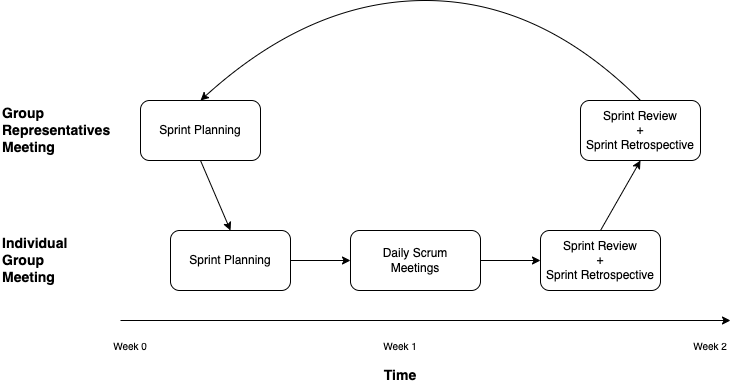
\includegraphics[width=\textwidth]{common/figures/Scrum_of_scrums_schedule.png}
    \caption{A figure depicting the events in a scrum sprint, divided between the big scrum of scrums group and the smaller scrum groups.}
    \label{fig:scrum-of-scrums-events}
\end{figure}


As mentioned, the multi-project focuses on both the GUI and Reveaal engine.
Because of this dual focus, we have two product owners: one product owner for the Reveaal teams and one for the GUI team.
The project's different product owners will help upholding the product backlog and update it if any changes appears. 
These changes are discussed during the scrum of scrums meetings, where the product owners can also be present.

The length of a sprint is measured against the length of the smaller scrum group's sprints.
Because of this, the average sprint length is two weeks.
Based on the length of the sprint, the scrum of scrums group has two meetings every two weeks. 
One meeting is for planning the upcoming sprint, and one is for sprint reviewing and retrospective at the end of a sprint.
These meetings, if possible, are held on the first Monday of a sprint, and the last Friday of a sprint, respectively.

% One for planing the upcoming sprint the first monday of the sprint, if possible and one meeting on last friday of the sprint, if possible.
% The last meeting's topics are always sprint reviewing and sprint retrospecting. 

\subsubsection{The Mutual Definition of Done}
To better facilitate multiple Scrum teams working on the same codebase, a Definition of Done (DoD) is necessary. The objective of defining a DoD is to have a shared agreement of when a feature is done, this shared definition was described in the first Scrum of Scrums meeting.

The definition we settled on was that every pull request to the GUI- and Reveaal-repositories' main-branches should be reviewed internally in the team as a draft, before it is sent out for an external review.
The external review consists of four different checks:
\begin{itemize}
    \item Ensure the new functionality described is implemented and works.
    \item Run a benchmark on the main- as well as the new functionalities branch.
    \item Check if the new code is properly documented. The I/O and panic criteria should be documented as well as what it does if functions are public.
    \item All tests should pass and if there is a new functionality it should be tested. It is up to the reviewers to judge if the tests are good enough.
\end{itemize}
Secondly the new functionality should be approved by two external reviewers.
%The external review consists of two people from other teams that follow a defined review guide which includes checks on functionality, performance, documentation, and tests.
If none of these areas are found lacking, and both reviewers approve of the changes, it is considered done.

It is worth noting that we have not made a formal definition for anything other than the code. However a review process for the collaborative part of the report exists. The review process is threefold, each Scrum team separately reviews the report. Thereafter each teams is assigned an area of responsibility, which is corrected and proof read. Lastly the original person/team who commented on the now corrected part, either accepts the change, or contacts the person who made it. After this process, the collaborative writing is considered done.
Any other DoD will be at the individual team's discretion to create.


% The mutual definition of DoD between the Scrum groups is:
% \begin{itemize}
%     \item Each increments should be reviewed by two students from the Scrum of Scrums.
%     \item Increments shall reviews internally in the group before making a pull request on Github.
%     \item If a increment is not reviewed in less than a day, the groups have failed to uphold their commitment to review other pull requests. 
%     \item Write code documentation that fits the written code. Such that having i/o variables defined, panic criteria and what the function descriptions.
%     \item It is up to the reviewers of the pull requests to say if the code is tested enough. 
% \end{itemize}



\section{Glossary}
In this section we outline and explain the main terms that are used throughout this report.

%\vspace{1em}
{\renewcommand{\arraystretch}{1.5}
\begin{xltabular}{\linewidth}[H]{>{\aautstyle}l|X}
    \endfirsthead
        %\multicolumn{2}{c}{\multirow{2}{*}{\footnotesize\textbf{Table \ref{tab:glossary}:} \textit{Continues on next page.}}}\\
        %\multicolumn{2}{c}{\multirow{2}{*}{\footnotesize\textbf{Table \ref{tab:glossary}:} Glossary.}}\\
    \endhead
    \endfoot
    \endlastfoot
    \multicolumn{2}{c}{\multirow{2}{*}{\footnotesize\textbf{Table \ref{tab:glossary}:} Glossary.}}\\
    TIOA & Timed Input/Output Automata are build upon two extensions to basic automata:
    \begin{enumerate}
        \item The addition of clocks to keep track of time.
        \item The addition of input/output actions.
    \end{enumerate} \\
    Clock & Clocks are used to represent time. They can be used in the edges' guards in a TIOA and can be re-assigned as an action. \\
    I/O actions & Input/Output actions are actions a TIOA can perform. Input actions originate from outside (the environment/other components), while output actions originate from within. \\
    Component & A Component is a subsystem, which is part of a bigger TIOA system, able to communicate with the other components through input/output actions. \\
    DBM & Difference Bound Matrices are a way to represent Zones (See Section \ref{sec:DBM} for more detail).\\
    Zone & Zones are the convex spaces where a clock-invariant evaluates to true. \\
    Federation & Federations are collections over DBMs (Section \ref{sec:DBM}). \\
    Specification &  A specification is a transition system where all of its states are input-enabled (See Section \ref{sec:TIOA})\\%Requirements that the model has to satisfy in order to verify the model.\\
    Refinement & An operator, denoted \texttt{<=} ($\leq$), verifying that more detailed models `coincide' within the abstract version of it. \\
    Conjunction & An operator, denoted \texttt{\&\&} ($\&\&$), that combines two or more specifications from the same component.\\
    Parallel Composition & An operator, denoted \texttt{||} ($||$), that combines two or more specifications from different components \\
    Quotient & An operator, denoted \texttt{\textbackslash\textbackslash} ($\backslash\backslash$), that calculates the missing component based on the current component and the given specification \\
    Pruning & An operation that gets rid of parts of the specifications that cannot be implemented.\\
    Reveaal & A backend-engine written in Rust for ECDAR, implementing TIOA model checking.
    \label{tab:glossary}
\end{xltabular}}


\chapter{Sprints}

This chapter outlines how we implemented the feature. Each section outlines a sprint where each will cover the sprint plans, along with the sprint review and retrospective. Beyond these sections each sprint will have some unique sections outlining elements related to that sprint only.

In the planning phase we look ahead and will try to determine how much work can be done in this sprint, along with trying to define the tasks in the backlog better.

In the reviewing phase we look back at our product and the plans for this sprint, which we review.


In the retrospective phase we look back at the developing process and reflect on the process.

\section{Sprint One}
The first sprint was spent getting a better understanding of the problem, the requirements, the theory, and the codebase. Beyond that, the Scrum Master from our team had to write, with the other Scrum Masters, some common sections about Ecdar and the work-method between groups, meaning the first sprint was spent doing quite a bit of research.

\subsection{Plans}
To get a better understanding of the problem a few things had to be researched:
\begin{itemize}
    \item Organization of the work inside our group as well as between the other groups.
    \item When the feature could be considered done.
    \item If there were any parts of the theory we should keep in mind.
    \item The different scenarios when a clock is redundant.
    \item Where in the codebase the feature should be implemented.
\end{itemize}

\subsection{Done criteria}
Our product owner gave us a definition of done which consists of
\begin{itemize}
    \item Our methods should remove some clocks in cases that we specify ourselves
    \item All refinement/consistency check tests pass successfully
    \item We can convincingly reason that our rules theoretically does not change the behavior in all cases. We can optionally formally prove it.
\end{itemize}

The done criteria are the main goals in this project, where the sprints are used to solve to-dos in the product backlog which is targeted at the criteria. The done criteria should therefore act as a guide for the scrum team where sprints are planned with the done criteria in mind. Each sprint review the scrum team will look at the done criteria to make sure they are on the right path, and how far they are from meeting the criteria.

\subsection{Relevant Theory}
While we are not creating additional theory, it is crucial to understand the relevant parts of the theory, and how to go about it. The primary theory we need to be aware of are DBMs (Section \ref{sec:DBM}), where we need to understand both how they are implemented, and what effect removing a clock has on them.

Theory-wise, when removing a clock, the corresponding row and column needs to be removed from the DBM. Luckily, the implementation is fairly straight forward. It is structured in a way that we only need to modify a hashmap with the clock definitions along with the guards they are used within and of course modifying the federation by either removing the clock, or ignore the clock by setting all of its constraints to either $\infty$ or $0$ as it fits.

\subsection{Scenarios} \label{scenarios}
When trying to reduce clocks there are multiple scenarios which can be looked into. One scenario is a clock being initiated but is not involved in constraints. The clock can in this situation be removed, as it does not violate any constraints. 

Another scenario is when components are combined using conjunction and parallel composition, one clock can affect the importance of the other resulting in the first clock becoming redundant. This can be done if the constraints becomes redundant when combining the clocks.

Another scenario where clocks from two components can be combined is if the two clocks both reset at the same time. Every situation needs to be analyzed to make sure that they reset at the same time, every time. Suppose in figure \ref{fig:tioa-scenario1} that the edges before and after the clock reset in each component only had output actions and no guards. If the two components were to be combined into one, the clocks could also be combined.  % they both only resets upon the same output action.


\begin{figure}[H]
    \centering
    \begin{tikzpicture}
        \node[state] (as) {$a_s$};
        \node[state, right=1cm of as] (1) {$a_1$};
        \node[state, right=2cm of 1] (2) {$a_2$};
        \node[state, right=1cm of 2] (af) {$a_f$};
        \node[state, below=.5cm of as] (bs) {$b_s$};
        \node[state, right=1cm of bs] (3) {$b_1$};
        \node[state, right=2cm of 3] (4) {$b_2$};
        \node[state, right=1cm of 4] (bf) {$b_f$};
        \draw   (1) edge[above, arrow] node{$o!$\hspace{1em}$x := 0$} (2)
                (3) edge[arrow, above] node{$o!$\hspace{1em}$y := 0$} (4)
                (as) edge[arrow] node[fill=white, font=\bfseries, pos=0.4]{\Large ?} (1)
                (bs) edge[arrow] node[fill=white, font=\bfseries, pos=0.4]{\Large ?} (3)
                (2) edge[arrow] node[fill=white, font=\bfseries, pos=0.4]{\Large ?} (af)
                (4) edge[arrow] node[fill=white, font=\bfseries, pos=0.4]{\Large ?} (bf)
        ;
    \end{tikzpicture}
    \caption{Two TIOA with clocks that reset at the same time.}
    \label{fig:tioa-scenario1}
\end{figure}

However in this scenario there are a few things to look out for, where the clocks cannot be combined. First scenario being if one of the components is cyclic like shown in figure \ref{fig:tioa-scenario2}. If the TIOA is cyclic we cannot prove that the two TIOAs will reset their clock at the same time. Therefore we can not prove that the model will be entirely the same when combining the two clocks. 

\begin{figure}[H]
    \centering
    \begin{tikzpicture}
        \node[state] (as) {$a_s$};
        \node[state, right=1cm of as] (1) {$a_1$};
        \node[state, right=2cm of 1] (2) {$a_2$};
        \node[state, right=1cm of 2] (af) {$a_f$};
        \node[state, below=1cm of as] (bs) {$b_s$};
        \node[state, right=1cm of bs] (3) {$b_1$};
        \node[state, right=2cm of 3] (4) {$b_2$};
        \node[state, right=1cm of 4] (bf) {$b_f$};
        \draw   (1) edge[above, arrow] node{$o!$\hspace{1em}$x := 0$} (2)
                (3) edge[arrow, above] node{$o!$\hspace{1em}$y := 0$} (4)
                (as) edge[arrow] node[fill=white, font=\bfseries, pos=0.4]{\Large ?} (1)
                (bs) edge[arrow] node[fill=white, font=\bfseries, pos=0.4]{\Large ?} (3)
                (2) edge[arrow] node[fill=white, font=\bfseries, pos=0.4]{\Large ?} (af)
                (4) edge[arrow] node[fill=white, font=\bfseries, pos=0.4]{\Large ?} (bf)
                (1) edge[arrow, bend right=2cm] node[above, font=\bfseries]{$o!$} (as)
        ;
    \end{tikzpicture}
    \caption{Two TIOAs where the clocks cannot be combined since one of them is cyclic.}
    \label{fig:tioa-scenario2}
\end{figure}


Another thing we need to check the components for is whether one of the components have the ability to make the output action that resets the clock before the other. An example of this scenario is shown in figure \ref{fig:tioa-scenario3} where the second component has the guard $y > 3$. Here we cannot be sure that the two clocks, $x$ and $y$, will reset at the same time, since the second component is dependent on a guard in order to reset.

\begin{figure}[H]
    \centering
    \begin{tikzpicture}
        \node[state] (as) {$a_s$};
        \node[state, right=2cm of as] (1) {$a_1$};
        \node[state, right=2cm of 1] (2) {$a_2$};
        \node[state, right=1cm of 2] (af) {$a_f$};
        \node[state, below=1cm of as] (bs) {$b_s$};
        \node[state, right=2cm of bs] (3) {$b_1$};
        \node[state, right=2cm of 3] (4) {$b_2$};
        \node[state, right=1cm of 4] (bf) {$b_f$};
        \draw   (1) edge[above, arrow] node{$o!$\hspace{1em}$x := 0$} (2)
                (3) edge[arrow, above] node{$o!$\hspace{1em}$y := 0$} (4)
                (as) edge[arrow] node[font=\bfseries, above]{$o!$} (1)
                (bs) edge[arrow] node[font=\bfseries, above]{$y>3\hspace{1em}o!$} (3)
                (2) edge[arrow] node[fill=white, font=\bfseries, pos=0.4]{\Large ?} (af)
                (4) edge[arrow] node[fill=white, font=\bfseries, pos=0.4]{\Large ?} (bf)
        ;
    \end{tikzpicture}
    \caption{Two TIOAs where the clocks $x$ and $y$ cannot be combined.}
    \label{fig:tioa-scenario3}
\end{figure}



\subsection{Codebase}
In the codebase for the Reveaal engine, where the solution for this project has to be implemented, we are going to work around the components. More specifically, before a component is assigned its clocks, an analysis of the component should be performed. 

There are however a question arising when the analysis happens before components are combined. How to know if a clock will become redundant before components are combined? The analysis has to take into account that components 

\subsection{Review}
This sprint had a big focus on researching and understanding the problem. Generally, it was successful. The Scrum Master finished the common sections for the report, while the group researched where they became more familiar with the codebase, theory, and the problem in general.

Theory-wise, the primary researched part was DBMs, since this is the more relevant to our problem of reducing clocks. This problems criteria for a solution was also given by the Product Owner, along with a few scenarios for when a clock can be reduced, with ranging difficulty.

Generally, the group did not find any elements of the problem making it seem either too much or too little to work with. The problem is naturally scalable in the sense that there are multiple scenarios for clock reduction, meaning we only need to implement the scenarios that seems doable within our capabilities and time constraint.



%Vi har fået en del content, 

%I forhold til. fællesskrivning:  Ecdar, Agile og Collaboration er done.

%Der er blevet skrevet om teori og kodebasen. 

%Teorimæssigt er. der skrevet om. TIOA og DMBs. Vi vil gerne have skrevet lidt mere om dbm (måske)? Der er skrevet om federations under dbm. Der mangler at blive skrevet om model checking

%Kodebasen er der skrevet lidt om, men nok til at informere læseren om hvor præcis klok analysen skal foregå i koden.

%Folk synes generelt, at opgaven er som vi regnede med.

%Hvor nemt er det at implementere i Rust? Vi skal have bedre overblik over kodebasen.

%Det advandcerede eksempel lyder spændende, men er mere kompliceret.

\iffalse
Mangler:
Omskriv model checking. BALINGO
Skriv om transition systems. Magnus
Define what a specification is. Magnus
Beslut om der er skrevet nok til dbm. Simon
Få review fra Martijn implementeret. Kira
Review. Loppe
\fi
\subsection{Retrospective}
This was the first sprint of this project, and generally caused some confusion. We were not completely aware when the sprint had actually started, meaning the start was a little hectic and poorly planned. Beyond that, a good deal of sickness haunted the group, meaning we were rarely present at the same time, making it hard to work together and agree on workload and -tasks.

Generally, we found some points to improve upon for next sprint:
\begin{itemize}
    \item Clearer communication regarding project status and work
    \item Better planing and definition tasks - Better usage of project boards
    \item Stick better to the sprint plan
\end{itemize}
These points will be considered heavily for the next sprint.

One element from our process which worked good was our daily sprint meetings, where we were all caught up on what we were doing. This fell a bit short though because of the reasons above.





%Der har været få fremmødte.
%Opgaver var lidt uklare, men det var også research opgaver.

%Det var uklart at sprintet var igang. Vi skal være tydelige i, at vi holder os til sprint planning.

%Det er godt at holde daily scrum/ sock check.

%Vi håndterede diskussion om arbejdstider ved at holde et møde. Vi aftalte at torsdag er arbejdsdag. Andet fravær skal du selv finde ud af at gøre op for. Vi skal arbejde lidt udenfor 'arbejdstiden'. Dette vil være velafgrænsede opgaver.

%arbejdsopgaver skal være mere veldefinerede. Vi vil, næste sprint, bruge project board og evaluere til næste sprint review. 
\section{Sprint Two}

\subsection{Plans}
The goal for the second sprint was identify the components that match the simple scenarios defined in section \ref{scenarios}. In the cases where the components match.



\subsection{Identifying Redundant Clocks}
We wanted to create a function, that we can use for identifying redundant clocks. We also wanted to create tests for this function. To do this the most efficient way, we split our group up in two sub groups working on the function and the tests. To do this we had to agree upon a function prototype. 

\subsection{Prototype}

The prototype we came up with was a function that takes in a component, which then returns a vector of redundant clocks, this can be seen in Listing \ref{lst:FindClockProto}. 

\begin{listing}
    \begin{rustcode}
        fn find_redundant_clocks(&self) -> Vec<RedundantClock> 
    \end{rustcode}
    \caption{Function prototype}
    \label{lst:FindClockProto}
\end{listing}
\begin{verbatim}
\end{verbatim}

The redundant clocks, contain infomation about the edges and locations where the clock is present, and also the reason for why it is declared redundant.

\begin{listing}
    \begin{rustcode}
    pub struct RedundantClock {
        clock: String,
        edge_indices: Vec<usize>,
        location_indices: Vec<usize>,
        reason: ClockReason,
        //updates: Option<Vec<Update>>,
    }
    \end{rustcode}
    \caption{Struct representing redundant clock}
    \label{lst:RedundantClock}
\end{listing}

The struct in Listing \ref{lst:RedundantClock} represent a redundant clock, where the field \texttt{clock} represent that clock key, that is used to access the clocks index in the component. This will be useful, when we implement a clock remover. \texttt{edge\_indices} and \texttt{location\_indices}, tell us where the clocks are used. 

The field \texttt{reason}, is a \texttt{ClockReason} enum, which describes the reason why a clock reduction operation was performed. The options are:
\begin{description}
\item[\texttt{Duplicate}] The clock was removed because it was exactly equivalent to another clock.
\item[\texttt{Unused}] The clock could be removed because it was never used in a guard or invariant.
\end{description}

\texttt{ClockReason} will also be used to send information to the GUI, of why it was removed.

Defining our data structures and function prototype, before beginning on the implementation allows us to create the implementation and testing of the function and data structures, simultaneously. 

\subsection{Implementation}

The redundant clock identifier, has been implemented in the component type's \texttt{block}, as it performs this analysis on it self.

%
%funktion skal have et component. Retunerer et array af strings som identificerer de clocks, som kan fjernes. 
%
%Derudover skal der være en enum som fortæller hvorfor den kan %fjernes. Dette kan kommunikeres over gRPC
%
%
%Når vi fjerner clocks skal vi nogle gange fjerne den, og andre %gange replace den med en clock som er identisk.
%
%
%
%\begin{verbatim}
%enum ClockOptimizationReason {
%    Redundant {
%        replaced_by_clock: String
%    },
%    Unused
%};
%
%struct ClockOptimization {
%    target: String;
%    reason: ClockOptimizationReason
%}
%
%fn find_optimizeable_clocks(component: &Component) -> %Vec<ClockOptimization>;
%
%fn find_removable_clocks(component: &Component) -> %Vec<ClockRemoval>;
%
%fn remove_clocks(component: &mut Component, clockOptimization: %&Vec<ClockOptimizationReason>);
%\end{verbatim}
%
%
%
%\begin{verbatim}
%enum ClockReason {
%    Duplicate(String),
%    Unused
%}
%
%struct RedundantClock {
%    clock: String,
%    edges: Vec<usize>,
%    locs: Vec<usize>,
%    reason: ClockReason,
%}
%
%fn find_redundant_clocks(&self) -> Vec<RedundantClock>;
%\end{verbatim}


\subsection{Testing Strategy}
By the end of any sprint, the output or the result should be an increment that improves product. As declared in the agile manifesto (SOURCE), the code that was produced should be working. The meaning of the word 'working' in this context is twofold: 

The increment should meet the definition of done(SCRUM). This first meaning of 'working' implies that the feature or improvement that was developed should meet the requirements for that feature. The act of checking if software meets its requirements is called \emph{validation testing}.

The second meaning of 'working' is that the implementation does not break in unexpected ways. This is sometimes referred to as \emph{defect testing}.

Developers are responsible for delivering working software so they require some heuristic that can inform them on the state of the code base. Automated testing is one such heuristic. For each feature that is introduced, there should be automated tests that validate that it is in fact working.

Automatic validation testing is a \emph{black box} test. Black box testing entails providing the system an input and the system must then return the correct output. The only thing of concern in this test is that the output should match an expected value. How this output is produced is not relevant to the test.


\paragraph{Unit Tests}
Unit testing is a kind of defect testing where a single \emph{unit} is isolated and tested by itself. A unit in this case refers to some small piece of the code base that is logically separated from other parts of the code base. In a object oriented language, this unit might be a class. Otherwise it might be a module that exposes some functions that can be used elsewhere. The unit test should be able to reveal any undesirable behavior that a given unit exhibits by itself. 

The test cases for unit tests of clock reduction are described below. These test cases are selected to test every aspect of the feature.

\paragraph{Unused clocks}
If a clock is never used in any guard in a component, it is technically unnecessary and it can always be removed.


\paragraph{Redudant clocks}
Two clocks that always reset at the same time are considered redundant and one of them can be removed. Guards and cycles can prevent clocks from being combined.

\paragraph{Combined}
A component can contain clocks that are unused as well as clocks that are duplicates. These have to be detected and reduced correctly.


\subsection{Acceptance Tests}




\subsection{Review}
\todo{Write friday 14/10}

\subsection{Retrospective}
\todo{Write friday 14/10}
\section{Sprint Three}


\subsection{Plans}
\todo{Write friday 17/10}

\subsection{Review}
\todo{Write friday 28/10}
\subsection{Retrospective}
\todo{Write friday 28/10}
\section{Sprint Four}


\subsection{Plans}
\todo{Write friday 31/10}

\subsection{Review}
\todo{Write friday 11/11}
\subsection{Retrospective}
\todo{Write friday 11/11}



%\chapter{Problem Statement}
\section{Summary of whatever the analysis said}
\section{Problem Statement}
\section{Delimitation}
\section{Requirements}
\section{Method}
%\chapter{Design}
%\chapter{Implementation}
\chapter{Test and Evaluation}
\chapter{Discussion}

\chapter{Summary of Findings}
\section{Method}
\section{Design}
\section{Implementation}
\section{Test and Evaluation}

\chapter{Conclusion}
\chapter{Future Work}
\bibliography{bibliography/bibliography, common/common.bib}
\chapter{Appendix}
{\aaufont
\begin{landscape}
    \chapter{Requirements Table}
    \begin{adjustwidth}{0pt}{0pt}
    \renewcommand{\arraystretch}{1.7}
    \begin{xltabular}{\linewidth} { l X X X X l}
    \tpagestyle{Ref. no.} & \tpagestyle{Summary} & \tpagestyle{Source(s)}  & \tpagestyle{Rationale} & \tpagestyle{Success criteria} & \tpagestyle{Importance}\\
     \hline
     \endfirsthead
    
    % \multicolumn{4}{c}{Continuation of Table}\\
    \textbf{Ref.nr.} & \textbf{Summary} & \textbf{Source(s)} & \textbf{Rationale}  & \textbf{Success criteria} & \textbf{Importance} \\
     \hline
     \endhead
    
    \multicolumn{6}{c}{Table continues on next page}\\
     \endfoot
    
     \multicolumn{6}{c}{End of Requirements Table}\\
     \endlastfoot
        F-1 & Summary & Where does the requirement come from? & Why is this a requirement & When do we know that this requirement is successfully implemented &  Must have\\  
        
       \end{xltabular}
    \end{adjustwidth}
    \end{landscape}
}


\end{document}